\documentclass[a4paper]{report}
\usepackage[utf8]{inputenc}
\usepackage[T1]{fontenc}
\usepackage{textcomp}

\usepackage{url}

% \usepackage{hyperref}
% \hypersetup{
%     colorlinks,
%     linkcolor={black},
%     citecolor={black},
%     urlcolor={blue!80!black}
% }

\usepackage{graphicx}
\usepackage{float}
\usepackage[usenames,dvipsnames]{xcolor}

% \usepackage{cmbright}

\usepackage{amsmath, amsfonts, mathtools, amsthm, amssymb}
\usepackage{mathrsfs}
\usepackage{cancel}

\newcommand\N{\ensuremath{\mathbb{N}}}
\newcommand\R{\ensuremath{\mathbb{R}}}
\newcommand\F{\ensuremath{\mathscr{F}}}
\newcommand\Z{\ensuremath{\mathbb{Z}}}
\renewcommand\O{\ensuremath{\emptyset}}
\newcommand\Q{\ensuremath{\mathbb{Q}}}
\newcommand\C{\ensuremath{\mathbb{C}}}
\let\implies\Rightarrow
\let\impliedby\Leftarrow
\let\iff\Leftrightarrow
\let\epsilon\varepsilon

% horizontal rule
\newcommand\hr{
    \noindent\rule[0.5ex]{\linewidth}{0.5pt}
}

\usepackage{tikz}
\usepackage{tikz-cd}

% theorems
\usepackage{thmtools}
\usepackage[framemethod=TikZ]{mdframed}
\mdfsetup{skipabove=1em,skipbelow=0em, innertopmargin=5pt, innerbottommargin=6pt}

\theoremstyle{definition}

\makeatletter

\declaretheoremstyle[headfont=\bfseries\sffamily, bodyfont=\normalfont, mdframed={ nobreak } ]{thmgreenbox}
\declaretheoremstyle[headfont=\bfseries\sffamily, bodyfont=\normalfont, mdframed={ nobreak } ]{thmredbox}
\declaretheoremstyle[headfont=\bfseries\sffamily, bodyfont=\normalfont]{thmbluebox}
\declaretheoremstyle[headfont=\bfseries\sffamily, bodyfont=\normalfont]{thmblueline}
\declaretheoremstyle[headfont=\bfseries\sffamily, bodyfont=\normalfont, numbered=no, mdframed={ rightline=false, topline=false, bottomline=false, }, qed=\qedsymbol ]{thmproofbox}
\declaretheoremstyle[headfont=\bfseries\sffamily, bodyfont=\normalfont, numbered=no, mdframed={ nobreak, rightline=false, topline=false, bottomline=false } ]{thmexplanationbox}


\declaretheorem[numberwithin=chapter, style=thmgreenbox, name=Definition]{definition}
\declaretheorem[sibling=definition, style=thmredbox, name=Corollary]{corollary}
\declaretheorem[sibling=definition, style=thmredbox, name=Proposition]{prop}
\declaretheorem[sibling=definition, style=thmredbox, name=Theorem]{theorem}
\declaretheorem[sibling=definition, style=thmredbox, name=Lemma]{lemma}



\declaretheorem[numbered=no, style=thmexplanationbox, name=Proof]{explanation}
\declaretheorem[numbered=no, style=thmproofbox, name=Proof]{replacementproof}
\declaretheorem[style=thmbluebox,  numbered=no, name=Exercise]{ex}
\declaretheorem[style=thmbluebox,  numbered=no, name=Example]{eg}
\declaretheorem[style=thmblueline, numbered=no, name=Remark]{remark}
\declaretheorem[style=thmblueline, numbered=no, name=Note]{note}

\renewenvironment{proof}[1][\proofname]{\begin{replacementproof}}{\end{replacementproof}}

\AtEndEnvironment{eg}{\null\hfill$\diamond$}%

\newtheorem*{uovt}{UOVT}
\newtheorem*{notation}{Notation}
\newtheorem*{previouslyseen}{As previously seen}
\newtheorem*{problem}{Problem}
\newtheorem*{observe}{Observe}
\newtheorem*{property}{Property}
\newtheorem*{intuition}{Intuition}


\usepackage{etoolbox}
\AtEndEnvironment{vb}{\null\hfill$\diamond$}%
\AtEndEnvironment{intermezzo}{\null\hfill$\diamond$}%




% http://tex.stackexchange.com/questions/22119/how-can-i-change-the-spacing-before-theorems-with-amsthm
% \def\thm@space@setup{%
%   \thm@preskip=\parskip \thm@postskip=0pt
% }

\usepackage{xifthen}

\def\testdateparts#1{\dateparts#1\relax}
\def\dateparts#1 #2 #3 #4 #5\relax{
    \marginpar{\small\textsf{\mbox{#1 #2 #3 #5}}}
}

\def\@lesson{}%
\newcommand{\lesson}[3]{
    \ifthenelse{\isempty{#3}}{%
        \def\@lesson{Lecture #1}%
    }{%
        \def\@lesson{Lecture #1: #3}%
    }%
    \subsection*{\@lesson}
    \testdateparts{#2}
}

% fancy headers
\usepackage{fancyhdr}
\pagestyle{fancy}

% \fancyhead[LE,RO]{Gilles Castel}
\fancyhead[RO,LE]{\@lesson}
\fancyhead[RE,LO]{}
\fancyfoot[LE,RO]{\thepage}
\fancyfoot[C]{\leftmark}
\renewcommand{\headrulewidth}{0pt}

\makeatother

% figure support (https://castel.dev/post/lecture-notes-2)
\usepackage{import}
\usepackage{xifthen}
\pdfminorversion=7
\usepackage{pdfpages}
\usepackage{transparent}
\newcommand{\incfig}[1]{%
    \def\svgwidth{\columnwidth}
    \import{./figures/}{#1.pdf_tex}
}

% %http://tex.stackexchange.com/questions/76273/multiple-pdfs-with-page-group-included-in-a-single-page-warning
\pdfsuppresswarningpagegroup=1

\author{Aamod Varma}
\setlength{\parindent}{0pt}


\title{MATH3012}
\author{Aamod Varma}
\usepackage{graphicx}
\graphicspath{ {./}}
\begin{document}
\maketitle


\section*{Keller and Trotter}
\section*{4.6}
\subsection*{Problem 2}
If we put $mn + 1$ pigeons in  $n$ holes then we will have to put at least $m + 1$  pigeons into the same hole. We can show this by contradiction, assume that each hole only has at most $m$ pigeons we have  $n$ holes, so we have a total of $m \times  n$ pigeons. However we are placing $nm + 1$ pigeons into the  $n$ holes which implies that all the holes can't have at most of $m$ pigeons, at least one must have more than $m$.




\subsection*{Problem 3}
It is not possible to put the 10 subsets in two holes such that there is no $3$ element subset  $S = \{a,b,c\}$ for which all pigeons from  $S$ go in the same hole. We need to put $10$ elements in $2$ holes, so we have at least one hole with $5$ elements - 5, two elements subsets of  $S$. However given $2$ elements there is only 1 way of constructing a 2 element subsets. This means that given a 2 element subset of the 5 in the hole, the 4 other subsets have at least one distinct number. We can construct $S$ that contains the 2 elements of the chosen subset and hat distinct number such that all of $S$ is in the hole.
\section*{5.9}



\subsection*{Problem 1}
a. 2

b. 4

c. 5 (1, 4, 6, 8, 9)

d. 1 - 5 - 6 - 2 - 3 - 10 - 4 - 7 - 1 is a cycle of length 8

e. 2

f. 3

g. 4 - 10 - 7 - 1 - 5 - 6


\subsection*{Problem 2}
\begin{tikzpicture}
    \draw (0,0) node[anchor=east] {1} -- (1,0) node[anchor=west] {2};
    \draw (2,0) node[anchor=east] {3} -- (3,0) node[anchor=west] {4};
    \draw (4,0) node[anchor=east] {5} -- (5,0) node[anchor=west] {6};
    \draw (6,0) node[anchor=east] {7} -- (7,0) node[anchor=west] {8};
\end{tikzpicture}

The above is a graph with 8 vertices where each vertex has odd degree  and there is no path of length 3.

\subsection*{Problem 3}
We are given degree 5, 4, 4, 2, 1, 1. We know that the sum of all the degree is twice the number of edges. This means that sum of all degrees is even. But we have, 
$$ 5 + 4 + 4 + 2 + 1 + 1 = 17 $$ 

which is an odd number. Hence such a graph is not possible.
\subsection*{Problem 4}


We have each team plays 7 distinct other teams. So we have total degree as $7 \times  7 = 49$. However this is not possible as the sum of degrees must be even.

Further it can't be that each team in a pool plays 5 other in the same pool as $7 \times  5 = 35$  which is not even. Hence it is NOT possible.
\subsection*{Problem 7}
We also see that $G_1$ and $G_3$ contain a cycle of length 3 while $G_4$ has 2 cycles of length 3 but $G_2$ doesn't have any cycle of length 3. So $G_2$ isn't isomorphic to any graph.

Similarly $G_4$ has 2 cycles of length 3 and none of the other have 2 cycles of length 3 which means $G_4$ isn't isomorphic to any other graph.

For pairs that are isomorphic we have, 
$$G_1 \cong G_3$$
defined by the function, 
$$ f(v_1)  = w_1, f(v_2) = w_3, f(v_3) = w_4, f(v_4) = w_2, f(v_5) = w_6, f(v_6) = w_5$$
\subsection*{Problem 8}

An eulerian circuit is (1, 6, 5, 3, 8, 4, 9, 2, 7, 12, 2, 10, 9, 3, 2, 11, 4, 1)

\subsection*{Problem 9}
All the degrees are even so its eulerian with the following walk, 
(l, a, b, l, d, h, m, g, n, m, i, d, j, m, c, i, f, e, a, k, f, c, j, l)


It is not Hamiltonian as any sequence that includes all the vertices needs to go through the cycle $m, n , g, m$ which would have to include  $m$ twice. But then it can't be a Hamiltonian cycle.
\subsection*{Problem 12}
We don't know for sure if either one is right. There is no direct way to determine if the graph is hamiltonian.
\subsection*{Problem 13}
We see that g-f-h-j-c-i-e-g forms an odd 7-cycle which means that it cannot have a 2 coloring. The graph has a chromatic number of 3 in our case.
\subsection*{Problem 14}
We see there is a 4-clique so our graph has chromatic number of 4.
\subsection*{Problem 15}

Let us define a graph theoretic model where each chemical is a vertex and is connected to another vertex if they cannot be stored in the same room. So the problem reduces to finding the chromatic number of our graph.


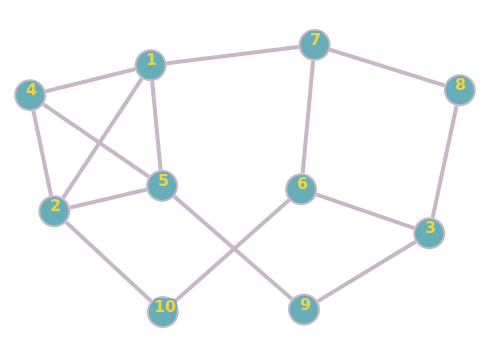
\includegraphics[scale=.5]{graph.png}


We see that there is a 4-clique and looking at the graph we see that the chromatic number is $4$. Hence we need at least 4 rooms.

\subsection*{Problem 17}

A tree with more than 1 vertex will have the chromatic number 2. This is because a tree does not have any cycles, and we know that any  graph with no odd cycle will have chromatic number of 2. We can start at the root of a tree and start assigning alternating colors to get a 2 coloring of any tree.
\subsection*{Problem 24}

The first ordering can be colored as follows,
\begin{align*}
    v_1, v_2 = 1, v_3, v_4 = 2, v_5, v_6 = 3, v_7, v_8 = 4
\end{align*}
The seconds can be done like this,
\begin{align*}
    (v_1, v_2, v_3, v_4) = 1 \text{ and } (v_5, v_6, v_7, v_8) = 0
\end{align*}
\subsection*{Problem 25}
The following is the interval graph
\begin{center}
\rotatebox[orgin=c]{90}{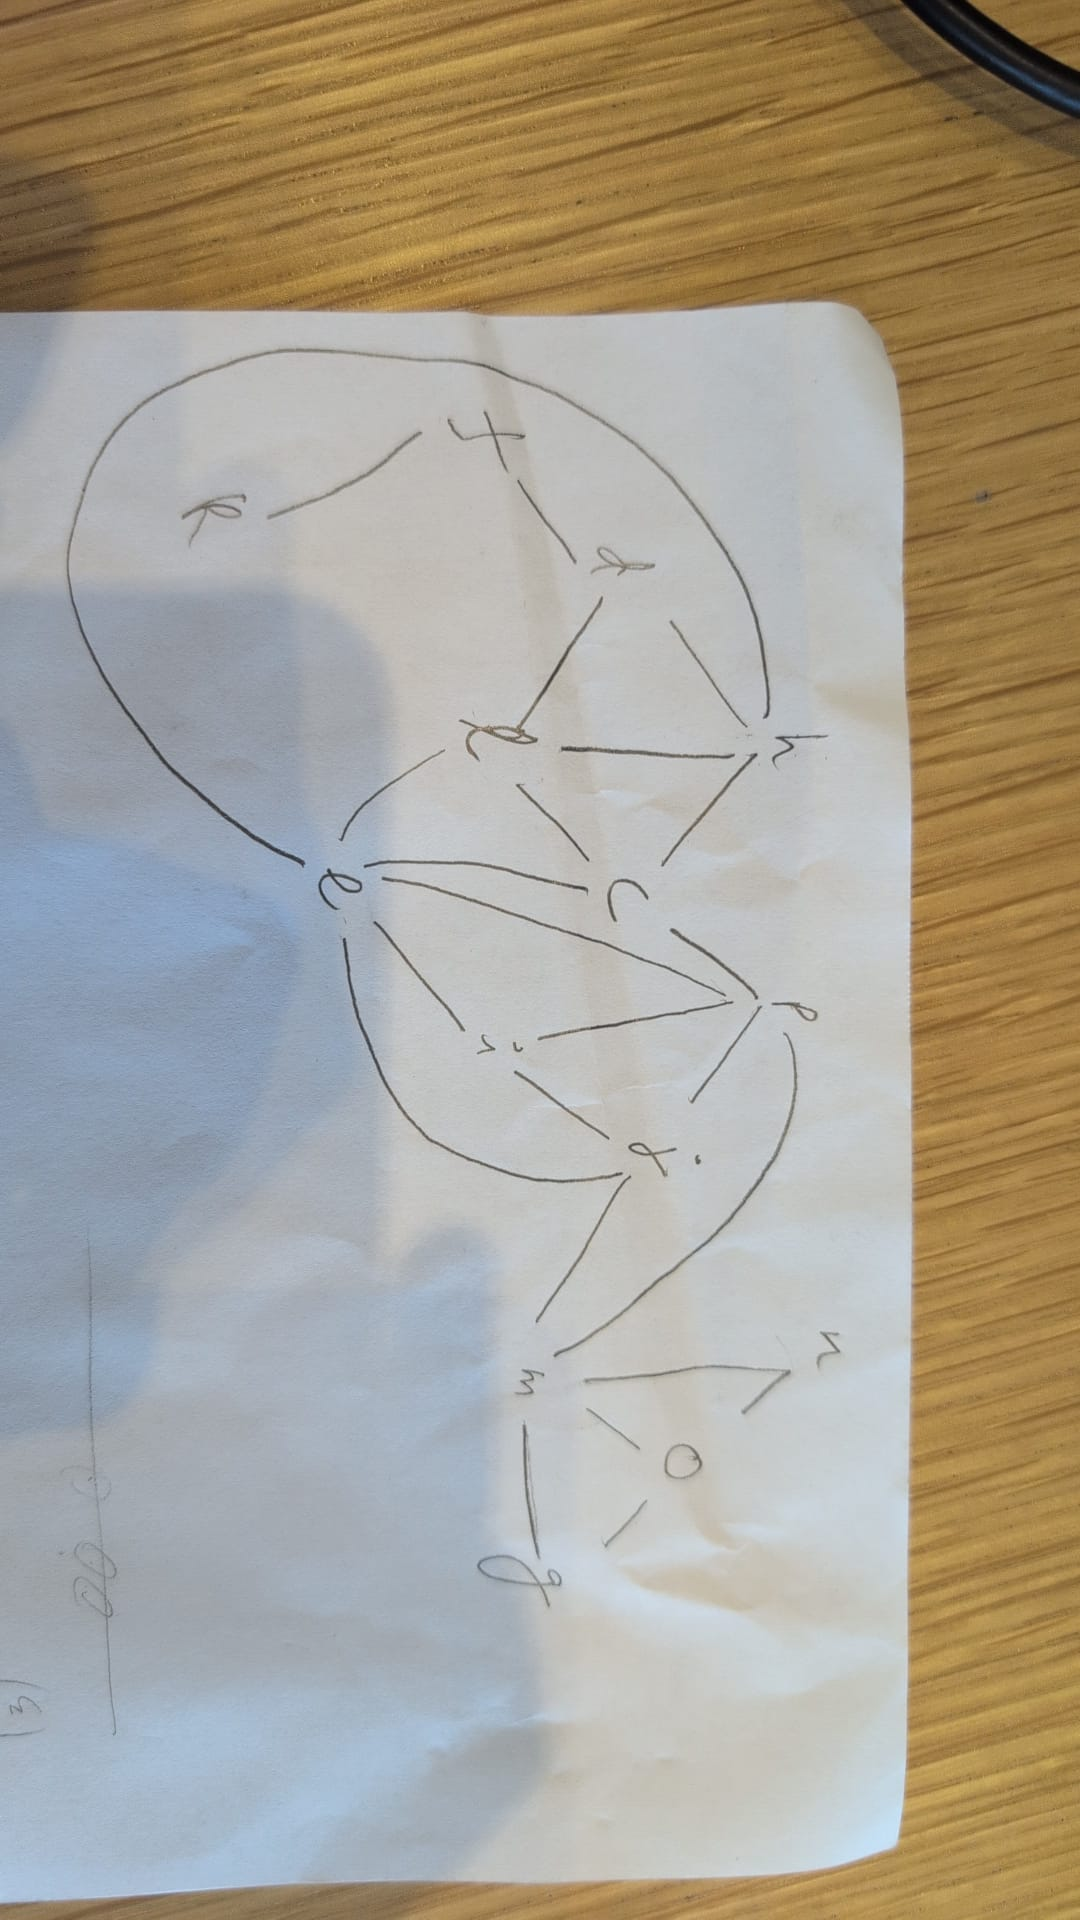
\includegraphics[scale=.1]{25}}
\end{center}
\subsection*{Problem 27}
a. We prove this by induction. Consider a graph with $n$ vertices. We start with $v_1$ and color it with a color. Now we assume true for case $n = k$. But we know that the max number of vertices is $D$. This means that there are at most $D$ neighbors with $D$ different colors. If this is the case that means that we can order $n = k + 1$ case with  the $D + 1$th color. So we showed that if true for  $n = k$ then it must be true for $n = k + 1$ completing the induction step.


b. Consider a graph with 2000 vertex where 1000 are on the left and 1000 on the right  paired with each other. Each node on the left is connected to all nodes on the right. The degree of each node is 1000. But the graph is bipartite (all left can be assigned 0 while all right can be assigned 1). So we show that the $D + 1 = 1001$ is not a tight upper bound.
\subsection*{Problem 29}
We see that the graph does not contain a $K_5$ or a $K_{3,3}$ hence this means it must be planar.


\subsection*{Problem 30}
\rotatebox[orgin=c]{90}{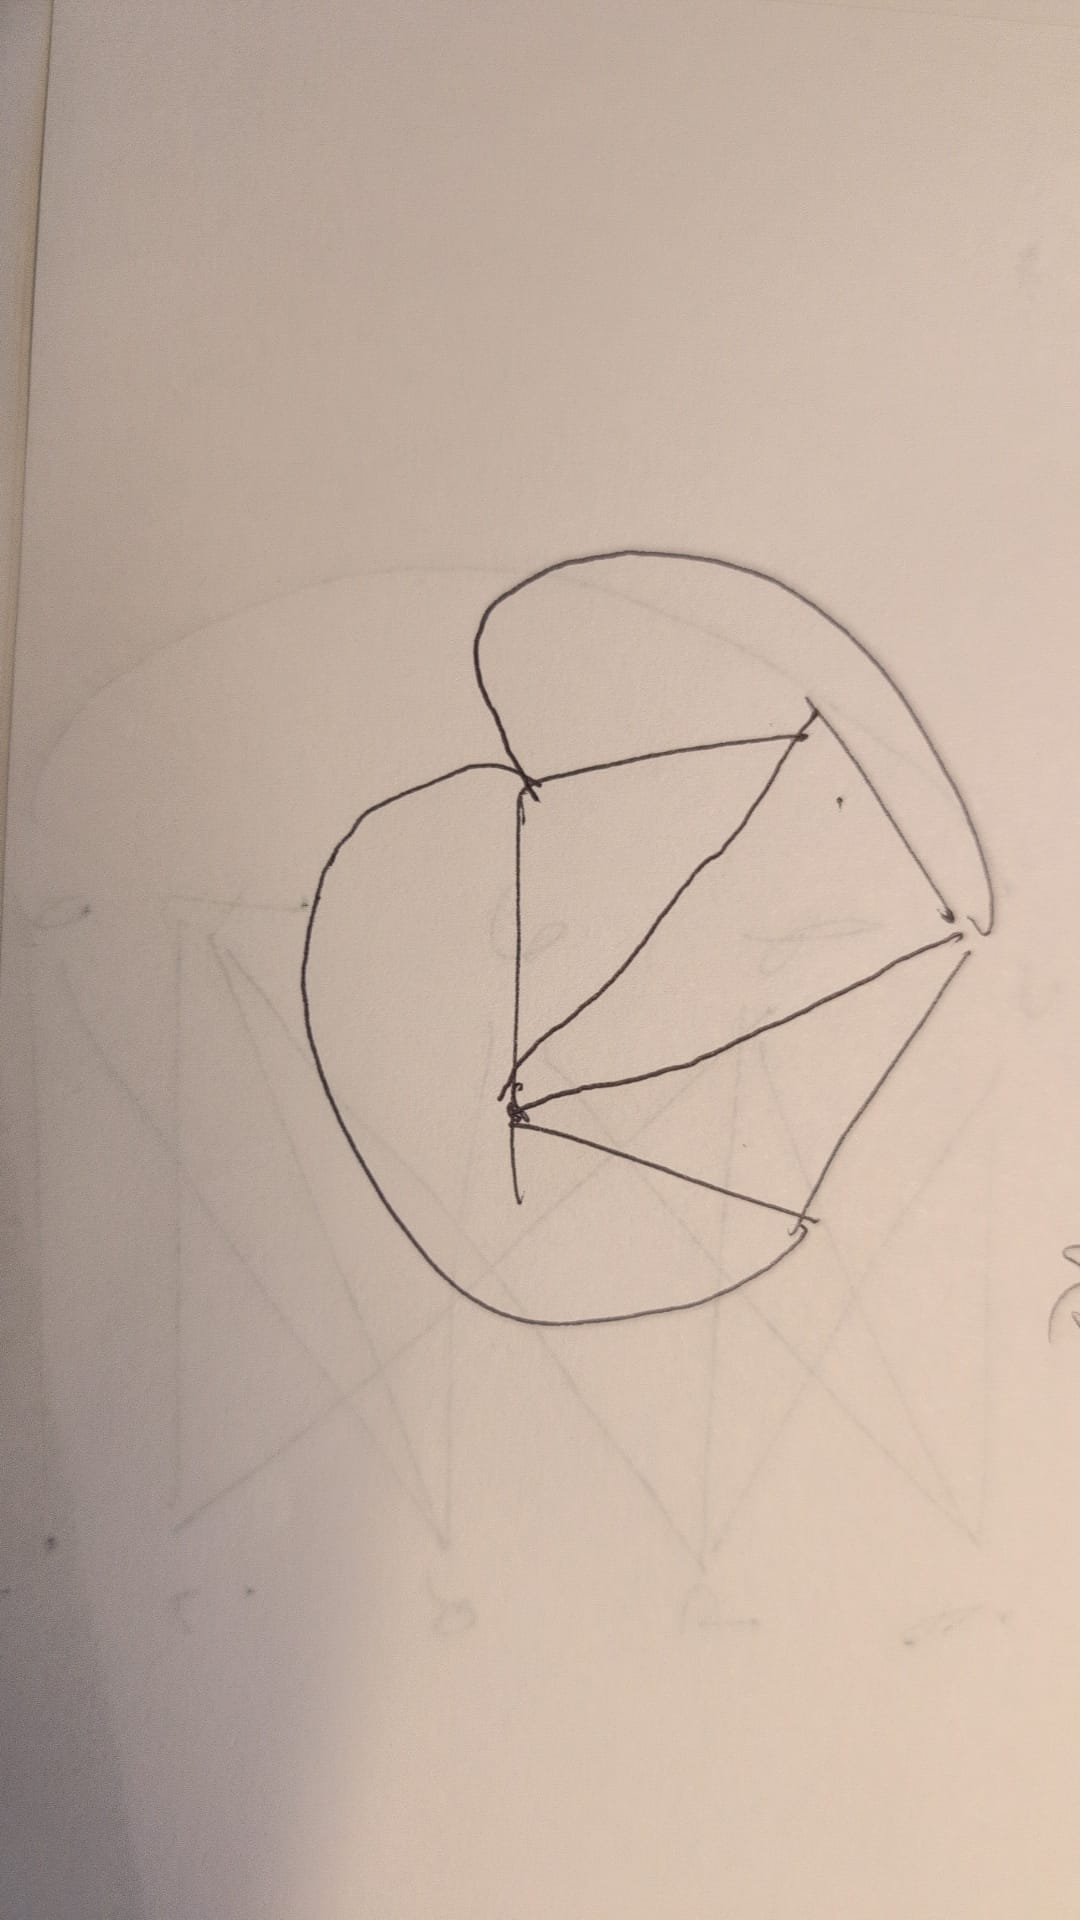
\includegraphics[scale=.1]{30}}

\subsection*{Problem 32}
Let us assume that is not the case - which means that every vertex has at least degree 6. Sum of degree would be $6n$ and the total edges would be  $6n /2 = 3n$. However we know that in a planar graph  of  $n$ vertices there are at most $3n - 6$ edges. But  $3n > 3n - 6$. Contradiction. So it must not be the case that all have at least 6 edges.

\subsection*{Problem 33}
c. cannot be the degree sequence of any graph as sum of degree is = 19

a. and e. can be planar as they satisfy they satisfy the $E \le 3n - 6$ criteria.

a. can be a tree as it has degree 1 leaves

b. must be the sequence that is the degree of an eulerian graph as it has all even degrees.

d. is the degree of graph that must be Hamiltonian as its a graph on 10 vertices with the minimum degree of 5.
\section*{Grimaldi}

\section*{Page 293}
\subsection*{Problem 3}
a. We need to show that $g$ dominates $f$. Or that $\exists m, k$ s.t., 
$$ |f(n)| \le m |g(n)| \qquad{\forall n \ge k}$$ 

If we choose $m = 200$ and  $k = 1$ we have,
\begin{align*}
    100 \log_2 (n) &\le 200 \frac{1}{2}  n\\
     \log_2 (n) &\le   n\\
     n &\le   2^{n}\\
\end{align*}
We know this is true for all $n \ge 1$. Hence we have, 

$$ |f(n)| \le m |g(n)| $$

for $m = 200, k = 1$

so we have  $f \in O(g)$


b. We have $f(n) = 2^{n}, g(n) = 2^{2n} - 1000$

We can just choose $m = 1$ and $k = 6$ for us to get,  
\begin{align*}
    2^{n} &\le (2^{n})^2 - 1000\\
    2^{6} &\le (2^{6})^2 - 1000\\
    64 &\le 4096 - 1000 = 3096\\
\end{align*}
And this will hold true for all $n > k$ as we know that  $2^{n}$ is an increasing function. So using definition we have, 
$$ f \in O(g) $$ 


c. We have $f(n) = 3n^2, g(n) = 2^{n} + 2n$

Here we can choose $m = 3$ so it is enough to show that, 
$$ n^2 \le  2^{n} + 2n $$  or even that, 
$$ n^2 \le 2^{n} $$ 

We can show that this is true by induction for all $n \ge 4$. Base case is obviously true. Assume true for any  $n =k$ we have,  
$$ k^2 \le 2^{k} $$ 

Consider $k + 1$ case we have,  
\begin{align*}
    (k + 1)^2 &\le 2^{k + 1}\\
    k^2 + 2k + 1 &\le 2 \times  2^{k}\\
\end{align*}

But from $n = k$ case we have $k^2 \le 2^{k}$ so, 
$$ k^2 + 2k + 1 \le 2^{k} + 2k + 1 $$ 

We know for $k \ge 4$ that  $2k + 1 \le 2^{k}$ so, 
$$ k^2 + 2k +  \le 2 \times  2^{k} $$ 

Hence induction step is over and we can conclude that, 
$$ f \in O(g) $$ 




\subsection*{Problem 6}
First let us assume that $f \in O(g)$ is true. This implies  $\exists m,k$ such that  $\forall n \ge k$,  
$$ |f(n)| \le m |g(n)| $$ 

However consider any $n > max(m, k)$ which is odd. We have,  $f(n) = n$ and  $g(n) = 1$ which gives us,  
$$ n \le m \times  1 $$ 

However we choose $n$ to be greater than $m$ but we have  $n \le m$ which is a contradiction. Hence  $f \in O(g)$ is not possible and we have $f \not \in O(g)$.

Similarly we can conclude that $g \not \in O(f)$

\section*{Page 300}
\subsection*{Problem 5}
a. In each loop iteration we perform 1 addition. Hence total addition is $n \cdot  1 = n = 5$. And in each loop iteration we perform 2 multiplications which is a total of $2n = 10$ multiplications.


b.  For the general case we have $n$ additions and  $2n$ multiplications.



\end{document}
